\documentclass{beamer}
\usetheme{Pittsburgh}
\beamertemplatenavigationsymbolsempty


\usepackage{amsmath}
\usepackage{amssymb}
\usepackage{bm} % For bold math symbols
\usepackage{graphicx}


\usepackage{subfigure}
\usepackage{multirow}
\usepackage{multicol}
\usepackage{color}
\usepackage{url}
\usepackage{hyperref}
\usepackage{listings}
\usepackage{algorithm}
\usepackage{physics}
% add image path
\graphicspath{{../Images/}}

\title{Weekly Updates\\
\tiny{Tuesday, 04/03/2025}}
\author{Andrea Bonifacio}
\date{}

\begin{document}

\begin{frame}
\titlepage
\end{frame}


\begin{frame}{Neural Modes Paper - Key Ideas}
    \begin{itemize}
        \item The paper wants to extend the concept of linear modes to ``neural modes''.
        \item The idea is to compute a non-linear correction of the displacement field, by having the network minimize the energy of the system.
        \item Once the network has been trained and learned the non-linear modes for any modal coordinate in the subspace, it can be extended to dynamics by using a finite difference scheme.
    \end{itemize}
\end{frame}



\begin{frame}
\frametitle{My implementation}
\begin{itemize}
    \item Computed eigenmodes by solving the generalized eigenvalue problem: \( K \mathbf{v} = \lambda M \mathbf{v} \)
    \begin{itemize}
        \item \( K \) is the stiffness matrix.
        \item \( M \) is the mass matrix.
        \item \( \mathbf{v} \) are the eigenvectors (modes).
        \item \( \lambda \) are the eigenvalues (squared frequencies).
    \end{itemize}
    \item Created a FEM environment compatible with PyTorch.
    \begin{itemize}
        \item Implemented sparse matrix operations in PyTorch.
        \item Enabled gradient computation through the FEM solver.
    \end{itemize}
\end{itemize}

\begin{figure}
    \centering
    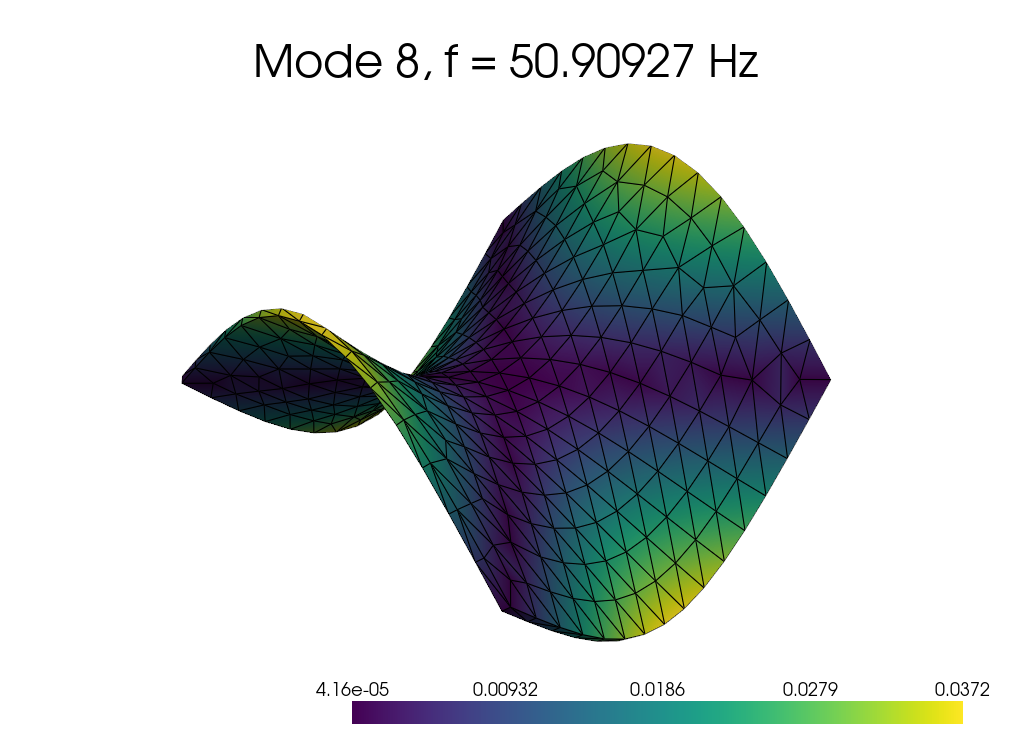
\includegraphics[width=0.45\textwidth]{Images/mode_9.png}
    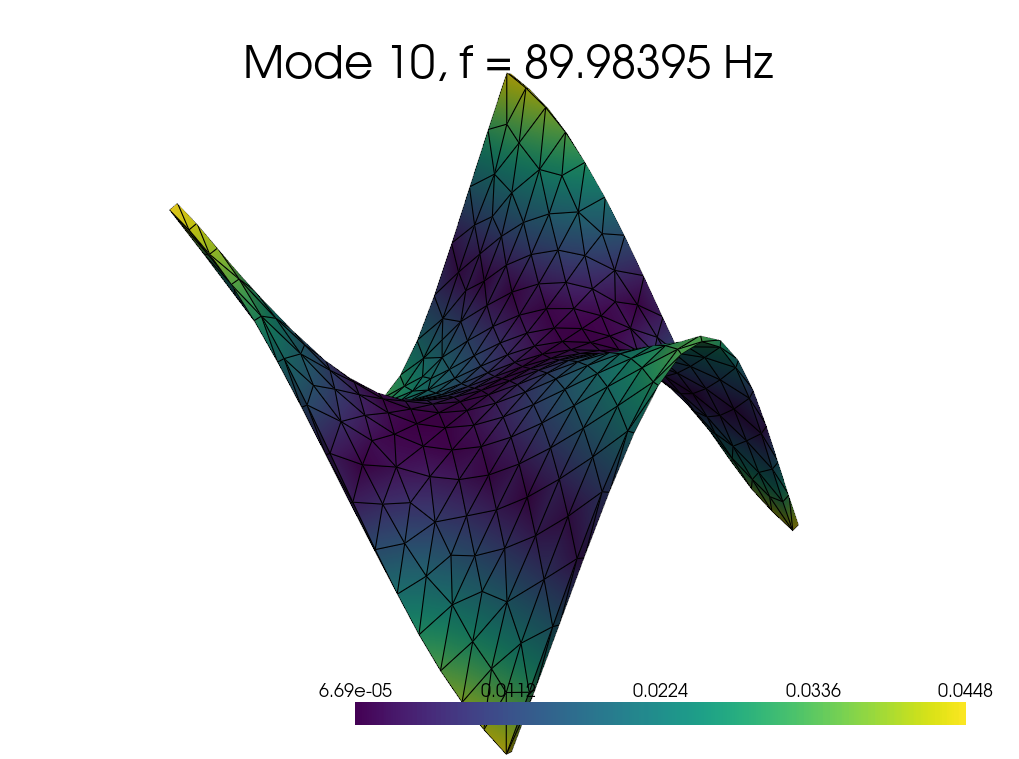
\includegraphics[width=0.45\textwidth]{Images/mode_10.png}
    \caption{Two eigenmodes of the mesh.}
    \label{fig:eigenmodes}
\end{figure}
\end{frame}

\begin{frame}
    \frametitle{Ideas - Neural Operators}
    \begin{itemize}
        \item Geometric Neural Operators \href{https://arxiv.org/pdf/2207.05209}{GNO}, where the mesh is deformed to a grid before being fed to the network.
        \item Super-Resolution Neural Operators \href{https://arxiv.org/pdf/2303.02584}{SRNO}, which is somewhat similar to our problem, but its output is a high-resolution tensor.
    \end{itemize}

    The main issue with our problem is that our target mesh needs to be of the same size as the input mesh, but our ground truth is a high-resolution mesh.
    

\end{frame}



\end{document}

